\chapter{Arhitektura i dizajn sustava}

		
	%	\textbf{\textit{dio 1. revizije}}\\

%		\textit{ Potrebno je opisati stil arhitekture te identificirati: podsustave, preslikavanje na radnu platformu, spremišta podataka, mrežne protokole, globalni upravljački tok i sklopovsko-programske zahtjeve. Po točkama razraditi i popratiti odgovarajućim skicama:}
%	\begin{itemize}
%		\item 	\textit{izbor arhitekture temeljem principa oblikovanja pokazanih na predavanjima (objasniti zašto ste baš odabrali takvu arhitekturu)}
%		\item 	\textit{organizaciju sustava s najviše razine apstrakcije (npr. klijent-poslužitelj, baza podataka, datotečni sustav, grafičko sučelje)}
%		\item 	\textit{organizaciju aplikacije (npr. slojevi frontend i backend, MVC arhitektura) }		
%	\end{itemize}

		\noindent Arhitektura sustava sastoji se od tri glavna dijela: 
		
		\begin{packed_item}
			\item Web preglednik 
			\item Web poslužitelj
			\item Baza podataka
		\end{packed_item}
		
		\textbf{Web preglednik} računalni je program koji korisnicima omogućuje  pristup internetu i pregled web stranica te interakciju s raznim online sadržajem. Korisnici koriste web preglednik za slanje zahtjeva web poslužitelju putem HTTP (eng. \textit{Hyper Text Transfer Protocol}) protokola i primanje odgovora u obliku HTML dokumenata koji se zatim interpretiraju i prikazuju. Osim pregledavanja web stranica, web preglednici omogućuju i izvođenje različitih aktivnosti kao što su ispunjavanje web obrazaca i prikaz slika i videozapisa.
		
		\textbf{Web poslužitelj} ključan je dio web aplikacija i internetskih servisa. Njegova je glavna uloga primanje, obrada i posredovanje zahtjeva koji dolaze od web preglednika korisnika. Web poslužitelj uspostavlja komunikaciju između klijenta (korisnika) i web aplikacije te osigurava ispravan protok informacija.
		
		\textbf{Web aplikacija} obrađuje zahtjeve korisnika. Nakon obrade zahtjeva, šalje se odgovor poslužitelju koji se korisniku prikazuje u web pregledniku. Obrada korisničkih zahtjeva najčešće uključuje određenu komunikaciju s bazom podataka npr. dohvaćanje, uređivanje ili brisanje podataka. \\
		
				
		Aplikacija je izgrađena korištenjem objektno orijentirane paradigme. Za poslužiteljski dio (\textit{backend}) korišten je radni okvir Java Spring Boot. Za izradu korisničkog sučelja (\textit{frontend}) koristi se open-source JavaScript biblioteka React. Odabrana su razvojna okruženja Visual Studio Code i IntelliJ IDEA.\\
		 
		 
		\noindent Korišteni Spring razvojni okvir koristi se MVC arhitekturom (eng. \textit{Model-View-Controller}). MVC arhitekturni obrazac razdvaja prezentaciju podataka, dohvat i manipulaciju podataka. MVC obuhvaća sljedeću podjelu uloga prikazanu i na slici \ref{arh}:
		
		\begin{packed_item}
			\item \textbf{Model} - sadrži razrede čiji objekti se obrađuju; služi za dohvat i manipulaciju podacima
			\item \textbf{View} - sadrži razrede čiji objekti služe za prikaz podataka; odlučuje kako će se dohvaćeni podaci prikazati
			\item \textbf{Controller} - prima zahtjeve za resursima od klijenta koje
			obrađuje i prosljeđuje; upravlja ostalim elementima sustava
		\end{packed_item}
		
		
		\begin{figure}[H]
			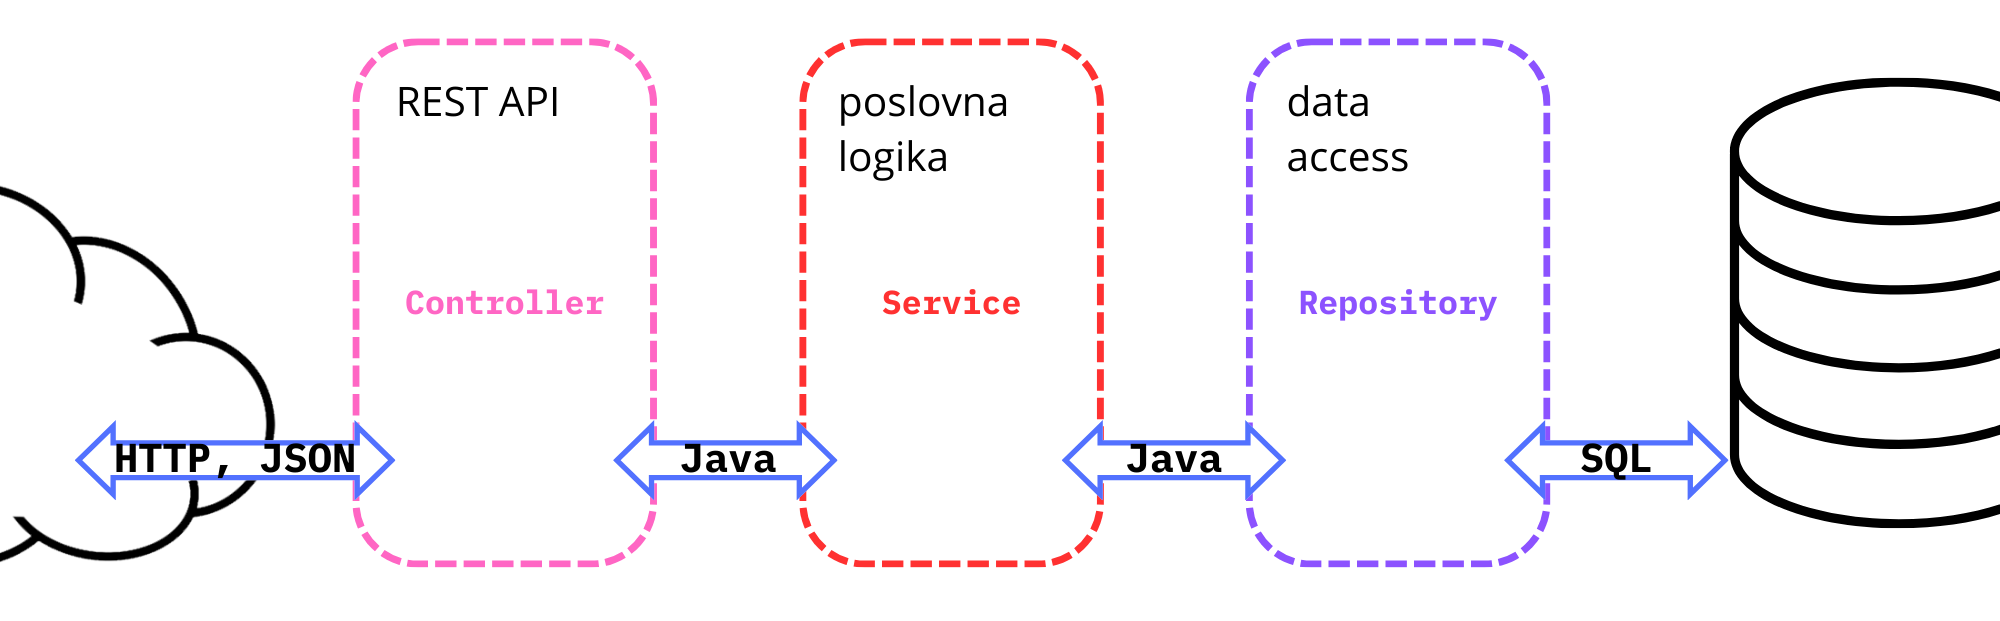
\includegraphics[width=\textwidth]{slike/mvc-arh.PNG}
			\centering
			\caption{Prikaz MVC arhitekture}
			\label{arh}
		\end{figure}
		
		\newpage
		
		\section{Baza podataka}
			
		Sustav koristi H2 relacijsku bazu podataka za organizaciju i pohranu različitih podataka. Organizacija temeljena na relacijskom modelu omogućuje lakšu manipulaciju podacima, pruža sigurnost i kontrolu nad podacima te osigurava trajno spremanje podataka. U sustavu baza podataka igra ključnu ulogu u pohrani informacija o korisnicima, događanjima i dodatnim informacijama o događanjima. Baza podataka ima sljedeće entitete:
		
		\begin{packed_item}
			\item Korisnik
			\item Dogadjanje
			\item Poveznica
			\item MedijskiSadrzaj
			\item Recenzija
			\item DolazakKorisnika
			\item Clanarina
			\item Pretplata
		\end{packed_item}
		
		\noindent Svaki od entiteta ima svoje atribute i jedinstveni primarni ključ koji osigurava jednoznačno identificiranje svakog zapisa. Baza podataka omogućuje brzu i jednostavnu pohranu, izmjenu i dohvat podataka, što je ključno za daljnju obradu podataka o događanjima.
		
			\subsection{Opis tablica}
			
				\noindent \textbf{Korisnik} Entitet sadrži sve relevantne informacije o registriranom korisniku aplikacije. Atributi id, korisnickoime, email, lozinka i tipkorisnika spremaju se za sve tipove korisnika sustava, dok se atributi adresa i placanjeclanarine odnose samo na organizatore i poprimaju vrijednost \textit{null} za tip korisnika Posjetitelj i Administrator.
				
				\begin{longtblr}[
					label=none,
					entry=none
					]{
						width = \textwidth,
						colspec={|X[8,l]|X[6, l]|X[20, l]|}, 
						rowhead = 1,
					}
					\hline \SetCell[c=3]{c}{\textbf{Korisnik}}	 \\ \hline[3pt]
					\SetCell{LightGreen}
					id & BIGINT	&  	jedinstveni identifikator korisnika  	\\ 
					\hline
					korisnickoime	& VARCHAR & korisničko ime\\ 
					\hline 
					email & VARCHAR & e-mail adresa korisnika  \\
					 \hline 
					lozinka & VARCHAR	&  lozinka korisničkog računa \\ 
					\hline 
					tipkorisnika & VARCHAR	& Posjetitelj, Organizator ili Administrator\\ 
					\hline 
					adresa & VARCHAR & adresa Organizatora\\ 
					\hline 
					placanjeclanarine & BOOLEAN	& plaća li Organizator članarinu\\ 
					\hline
				\end{longtblr}
				
				\noindent \textbf{Dogadjanje} Entitet omogućuje pohranu informacija o različitim događanjima koja se mogu organizirati. Atribut organizatorid strani je ključ koji se odnosi na korisnika koji je organizator događanja. Atribut cijenaulaznice sadrži informacije o cijeni ulaznica za događanje, a može biti i \textit{null} u slučaju da je događanje besplatno. 
				
				\begin{longtblr}[
					label=none,
					entry=none
					]{
						width = \textwidth,
						colspec={|X[8,l]|X[6, l]|X[20, l]|}, 
						rowhead = 1,
					} 
					\hline \SetCell[c=3]{c}{\textbf{Dogadjanje}}	 \\ \hline[3pt]
					\SetCell{LightGreen}
					iddogadjanja & BIGINT	&  	jedinstveni identifikator događanja  	\\ 
					\hline
					nazivdogadjanja	& VARCHAR & naziv događanja \\ 
					\hline 
					tipdogadjanja & VARCHAR & vrsta događanja  \\
					\hline 
					lokacijagodadjanja & VARCHAR & lokacija događanja \\ 
					\hline 
					vrijemedogadjanja & TIMESTAMP & datum i vrijeme događanja\\ 
					\hline 
					trajanje & DOUBLE & vremensko trajanje događanja\\ 
					\hline 
					\SetCell{LightBlue} organizatorid & BIGINT	& identifikator Organizatora \\ 
					\hline
					cijenaulaznice & DOUBLE	& cijena ulaznice događanja\\ 
					\hline
				\end{longtblr}
				
				\noindent \textbf{Poveznica} Entitet služi za pohranu podataka o poveznicama koje su povezane s određenim organizatorima događanja (strani ključ organizatorid). 
				
				\begin{longtblr}[
					label=none,
					entry=none
					]{
						width = \textwidth,
						colspec={|X[8,l]|X[6, l]|X[20, l]|}, 
						rowhead = 1,
					} 
					\hline \SetCell[c=3]{c}{\textbf{Poveznica}}	 \\ \hline[3pt]
					\SetCell{LightGreen}
					idpoveznice & BIGINT & jedinstveni identifikator poveznice  	\\ 
					\hline
					\SetCell{LightBlue} organizatorid & BIGINT	& identifikator Organizatora \\ 
					\hline
					link & VARCHAR	& poveznica na web stranice Organizatora\\ 
					\hline
				\end{longtblr}
				
				\noindent \textbf{MedijskiSadrzaj} Entitet omogućava pohranu različitih medijskih sadržaja koji su povezani s određenim događanjima, što omogućava organizatorima da dijele fotografije i videozapise povezane s njihovim događanjima.
				
				\begin{longtblr}[
					label=none,
					entry=none
					]{
						width = \textwidth,
						colspec={|X[10,l]|X[6, l]|X[20, l]|}, 
						rowhead = 1,
					} 
					\hline \SetCell[c=3]{c}{\textbf{MedijskiSadrzaj}}	 \\ \hline[3pt]
					\SetCell{LightGreen}
					idmedijskogsadrzaja & BIGINT & jedinstveni identifikator sadržaja  	\\ 
					\hline
					\SetCell{LightBlue} iddogadjanja & BIGINT	& identifikator događanja \\ 
					\hline
					medijskisadrzaj & LONGLOB & medijski sadržaj\\ 
					\hline
				\end{longtblr}
				
				\noindent \textbf{Recenzija} Entitet služi za pohranu recenzija koje korisnici mogu napisati za određena događanja u sustavu. Entitet omogućava korisnicima da izraze svoje mišljenje i ocjene događanja, čime se pruža povratna informacija organizatorima i drugim potencijalnim sudionicima.
				
				
				\begin{longtblr}[
					label=none,
					entry=none
					]{
						width = \textwidth,
						colspec={|X[8,l]|X[6, l]|X[20, l]|}, 
						rowhead = 1,
					} 
					\hline \SetCell[c=3]{c}{\textbf{Recenzija}}	 \\ \hline[3pt]
					\SetCell{LightGreen}
					idrecenzije & BIGINT	&  	jedinstveni identifikator recenzije\\ 
					\hline
					recenzijatekst & TEXT & tekst napisane  recenzije \\
					\hline
					ocjena & INT & dodijeljena ocjena događanja\\
					\hline 
					\SetCell{LightBlue} iddogadjanja & BIGINT & identifikator događanja\\
					\hline 
					\SetCell{LightBlue} idkorisnik & BIGINT & identifikator korisnika (autora recenzije)\\ 
					\hline
				\end{longtblr}
				
				\noindent \textbf{DolazakKorisnika} Entitet služi za praćenje iskazanog interesa korisnika za dolazak na određeno događanje. Atribut statusdolaska može poprimiti vrijednosti \textit{sigurno dolazim}, \textit{možda dolazim} i \textit{ne dolazim}.
				
				\begin{longtblr}[
					label=none,
					entry=none
					]{
						width = \textwidth,
						colspec={|X[9,l]|X[6, l]|X[20, l]|}, 
						rowhead = 1,
					} 
					\hline \SetCell[c=3]{c}{\textbf{DolazakKorisnika}}	 \\ \hline[3pt]
					\SetCell{LightGreen}
					iddolaskakorisnika & BIGINT	&  	jedinstveni identifikator dolaska  	\\ 
					\hline
					statusdolaska & VARCHAR & iskazani interes za dolazak \\ 
					\hline 
					\SetCell{LightBlue} iddogadjanja & BIGINT & identifikator događanja  \\
					\hline 
					\SetCell{LightBlue} idkorisnik & BIGINT & identifikator korisnika\\ 
					\hline
				\end{longtblr}
				
				\noindent \textbf{Clanarina} Entitet služi za praćenje informacija o članarinama koje organizatori moraju platiti kako bi imali mogućnost organiziranja događanja za koja se plaća ulaz. Entitet omogućava praćenje članarina koje su korisnici platili te pruža informacije o cijenama i datumima isteka vrijednosti članarine.
				
				\begin{longtblr}[
					label=none,
					entry=none
					]{
						width = \textwidth,
						colspec={|X[8,l]|X[6, l]|X[20, l]|}, 
						rowhead = 1,
					} 
					\hline \SetCell[c=3]{c}{\textbf{Clanarina}}	 \\ \hline[3pt]
					\SetCell{LightGreen}
					idclanarine & BIGINT	&  	jedinstveni identifikator članarine \\ 
					\hline
					\SetCell{LightBlue} idkorisnik & BIGINT & identifikator korisnika \\ 
					\hline 
					cijenaclanarine & DOUBLE & iznos cijene članarine  \\
					\hline 
					vrijedido & TIMESTAMP & datum i vrijeme isteka članarine\\ 
					\hline
				\end{longtblr}
				
				\noindent \textbf{Pretplata} Entitet služi za spremanje korisničkih postavki o automatskom slanju obavijesti o novim događanjima. Posjetitelji mogu odabrati postavke da im aplikacija automatski šalje obavijesti o najnovijim događanjima prema kriterijima vrsta (kategorija) događanja i područje (lokacija).  
				
				\begin{longtblr}[
					label=none,
					entry=none
					]{
						width = \textwidth,
						colspec={|X[8,l]|X[6, l]|X[20, l]|}, 
						rowhead = 1,
					} 
					\hline \SetCell[c=3]{c}{\textbf{Pretplata}}	 \\ \hline[3pt]
					\SetCell{LightGreen}
					idpretplata & BIGINT &  jedinstveni identifikator pretplate \\
					\hline 
					\SetCell{LightBlue} idkorisnik & BIGINT & identifikator korisnika \\ 
					\hline 
					kategorija & VARCHAR & kategorija za koju želi primati obavijesti\\
					\hline 
					lokacija & VARCHAR & lokacija za koju želi primati obavijesti\\ 
					\hline
				\end{longtblr}
				
				\newpage
				
			
			\subsection{Dijagram baze podataka}
				
				\begin{figure}[H]
					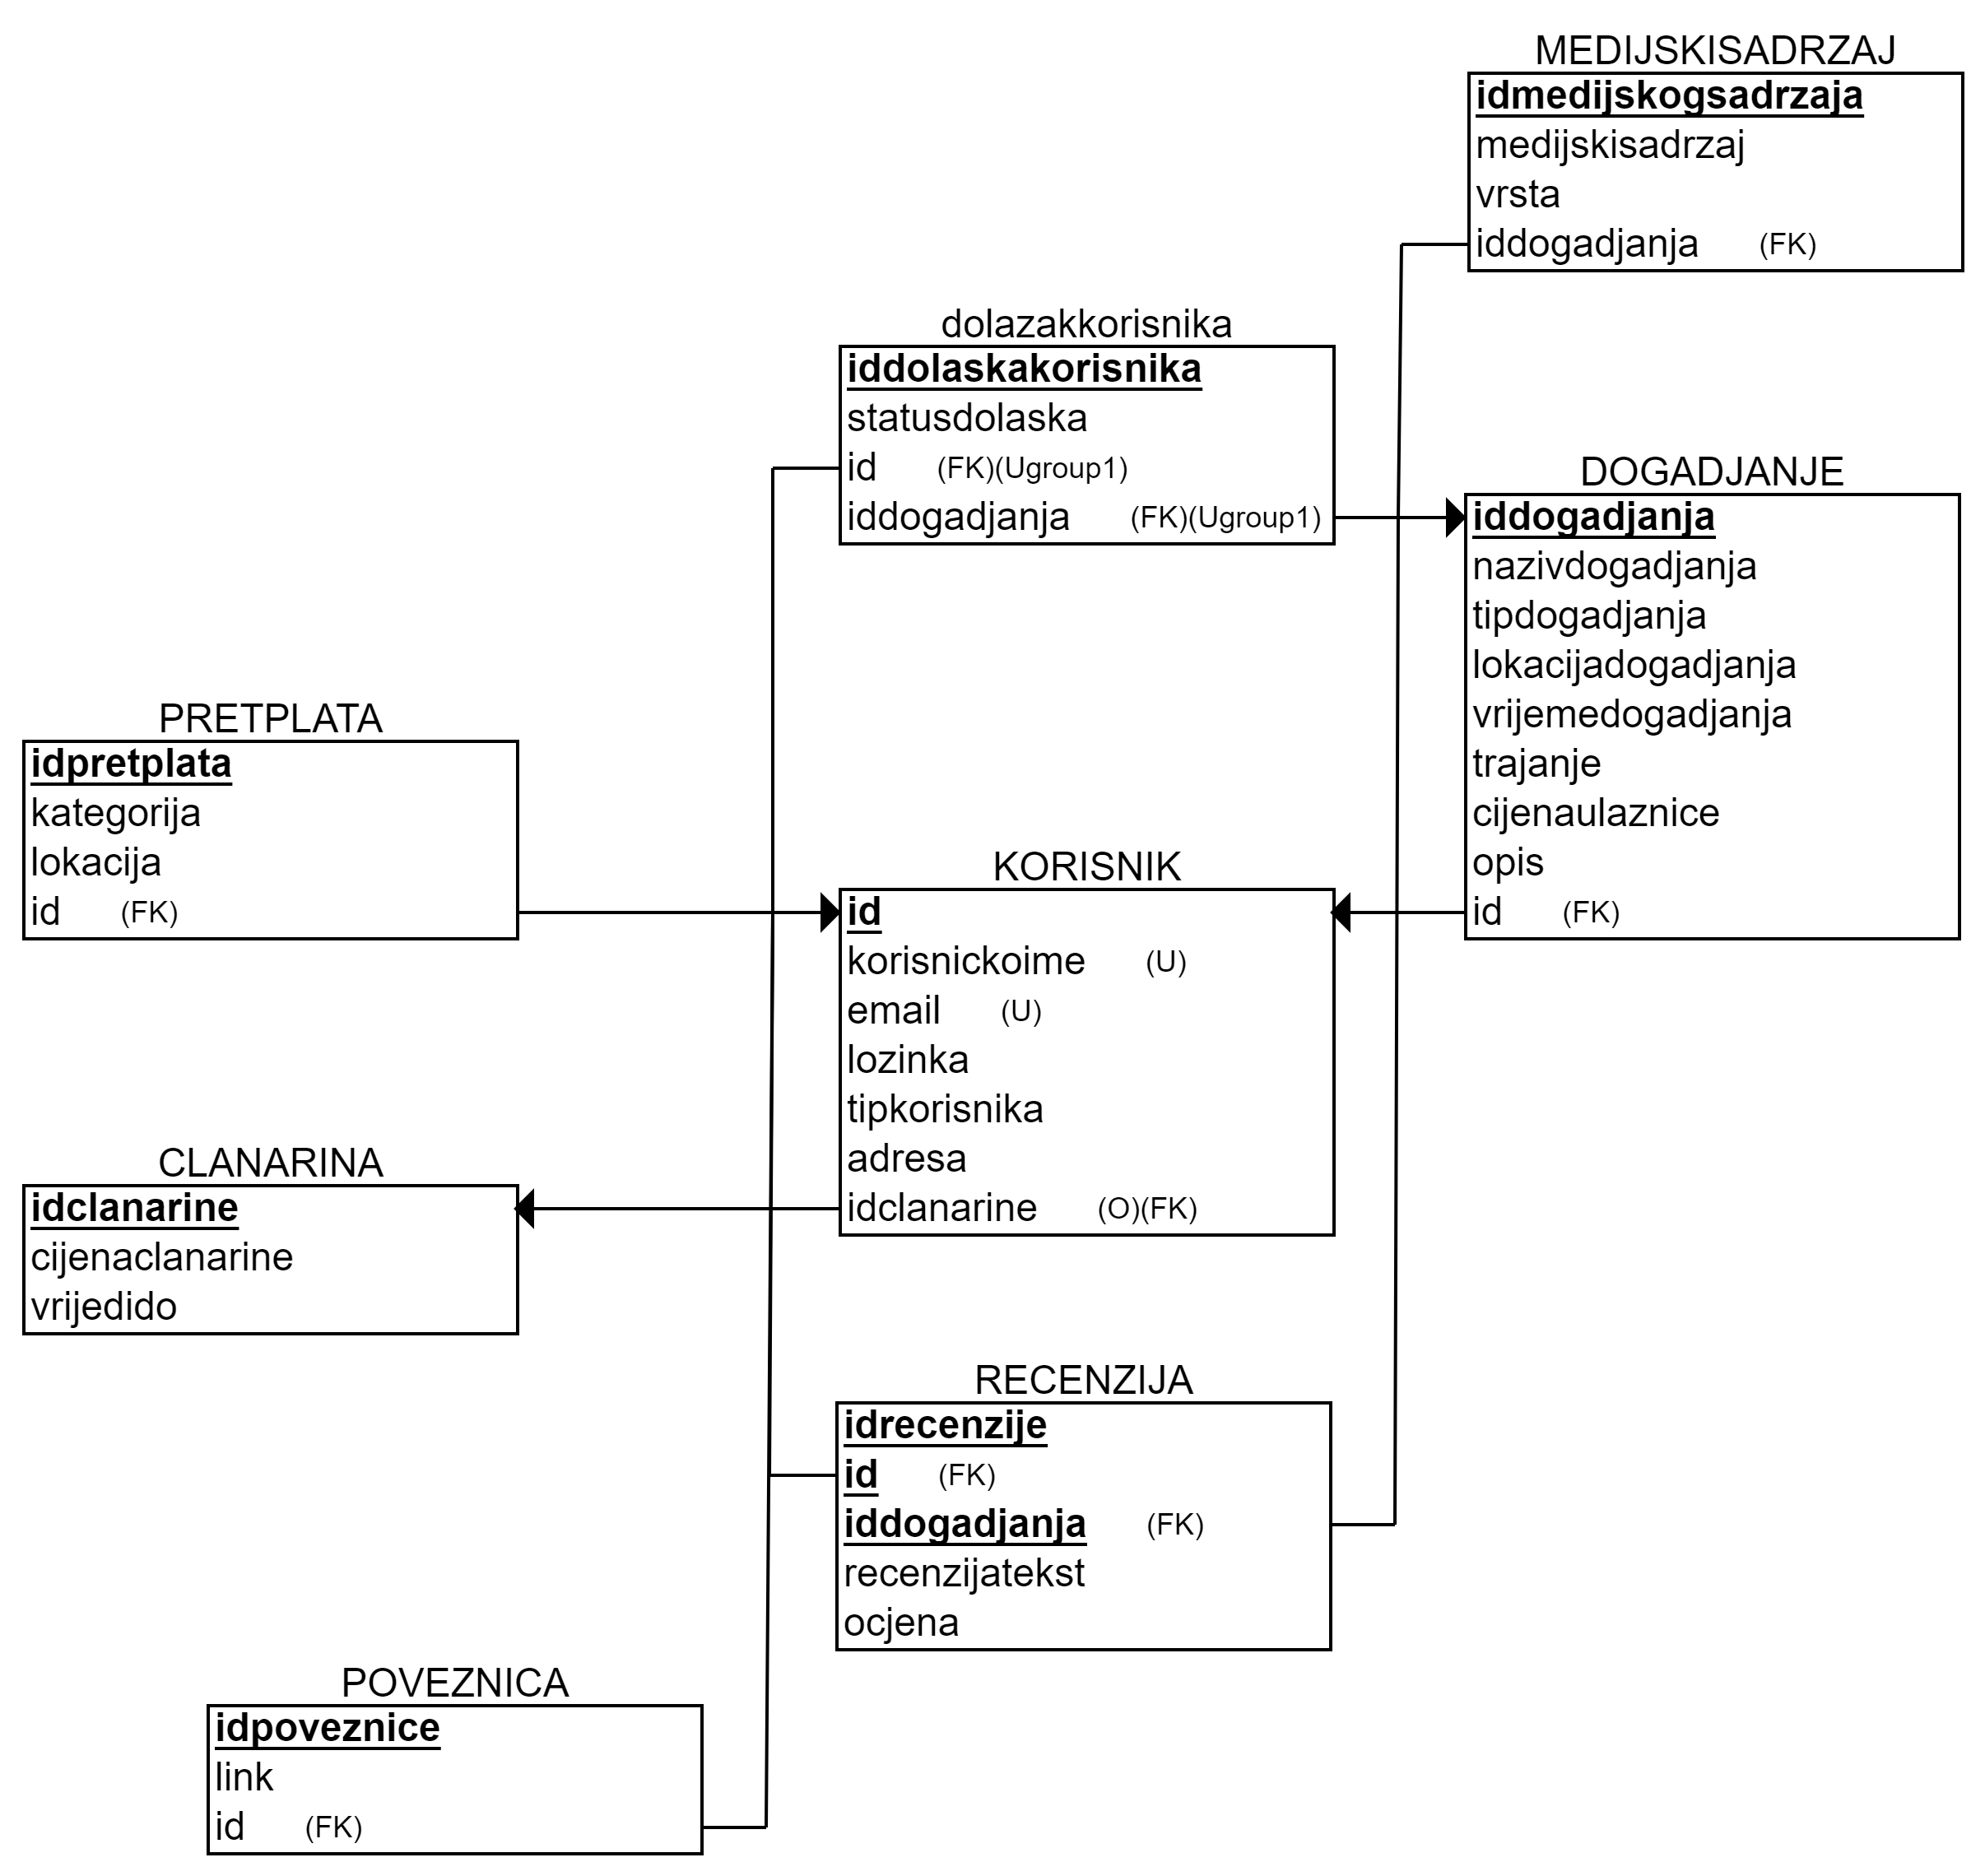
\includegraphics[width=\textwidth]{dijagrami/db_REL.png} 
					\centering
					\caption{Dijagram baze podataka}
					\label{fig:promjene}
				\end{figure}
				
				\newpage
				
				\begin{figure}[H]
					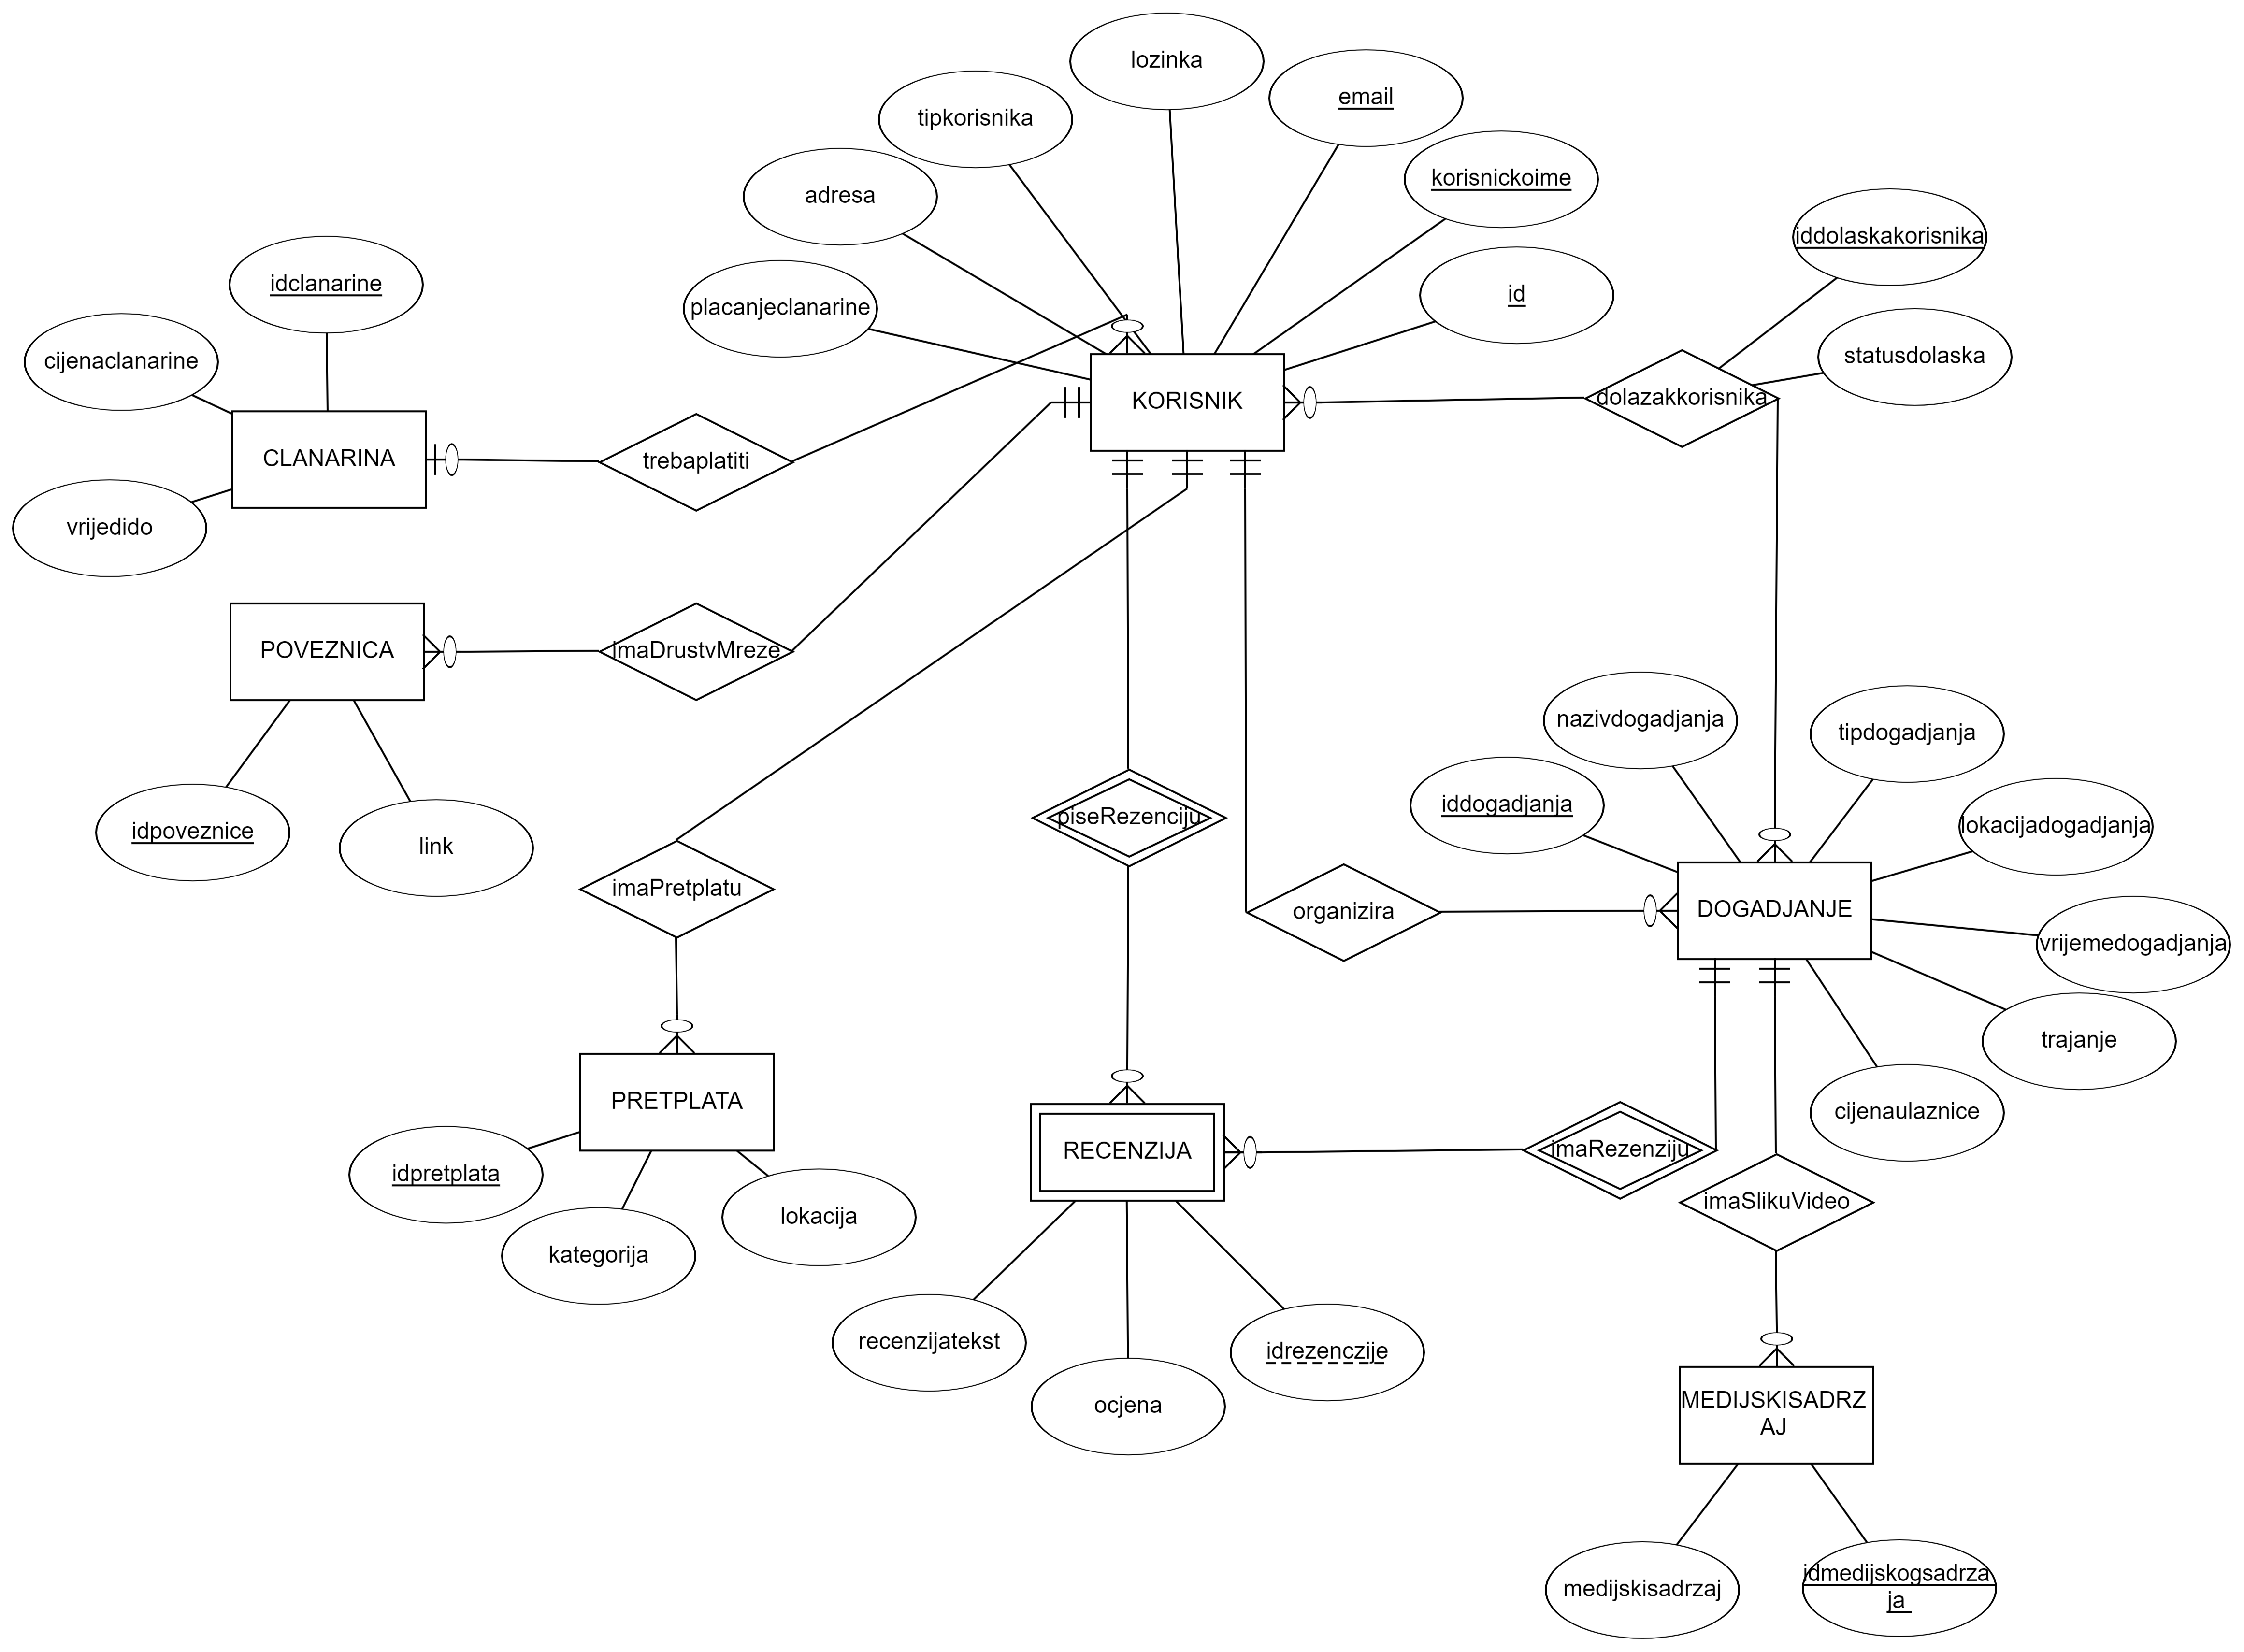
\includegraphics[width=\textwidth]{dijagrami/db_ER.png} 
					\centering
					\caption{ER dijagram baze podataka}
				\end{figure}
				
			\eject
			
			
		\section{Dijagram razreda}
		
		Dijagrami razreda prikazuju razrede u objektno orijentiranom sustavu, njihove atribute i
		metode te veze između razreda koji međusobno komuniciraju ili se nasljeđuju. Na slikama su prikazani razredi koji odgovaraju backend dijelu MVC arhitekture. Slika \ref{cd2} prikazuje sučelja koja pripadaju sloju Repository. Razredi prikazani na slici \ref{cd3} nasljeđuju Controller razred. Na slici \ref{cd5} prikazan je sloj Services, a na slici \ref{cd4} Data transfer objects. Razredi prikazani na \ref{cd1} predstavljaju entitete iz baze podataka. Članske varijable tih klase atributi su odgovarajućih entiteta baze podataka.

			\begin{figure}[H]
				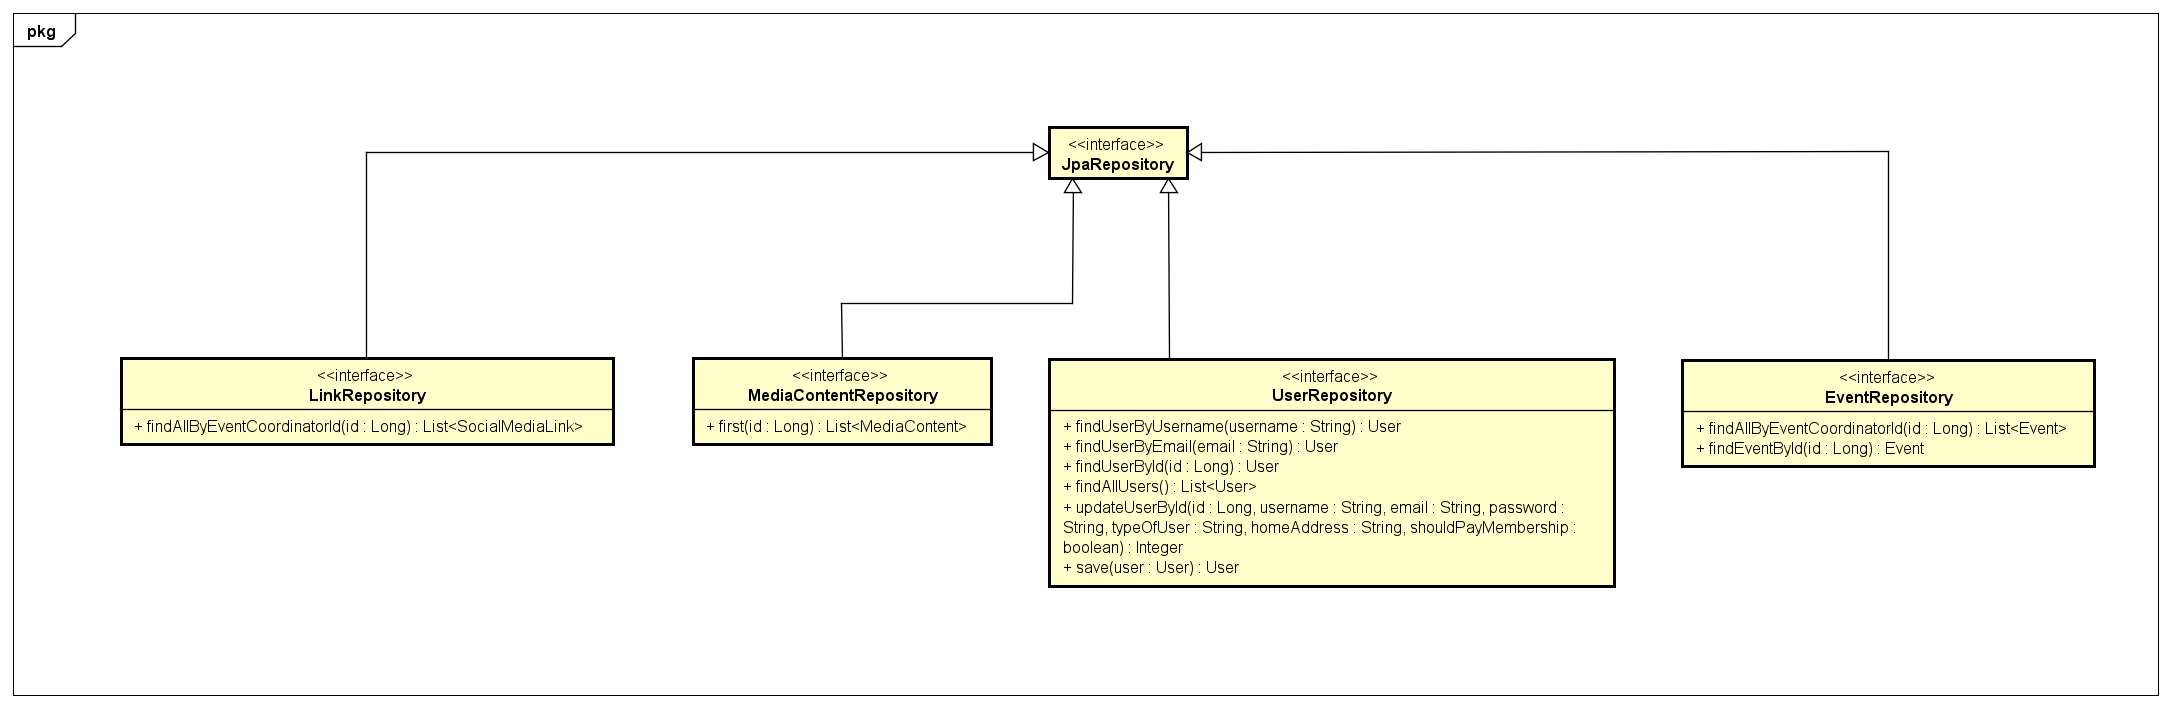
\includegraphics[width=\textwidth]{dijagrami/cd2.png} 
				\centering
				\caption{Dijagram razreda - Repository}
				\label{cd2}
			\end{figure}
			
			\begin{figure}[H]
				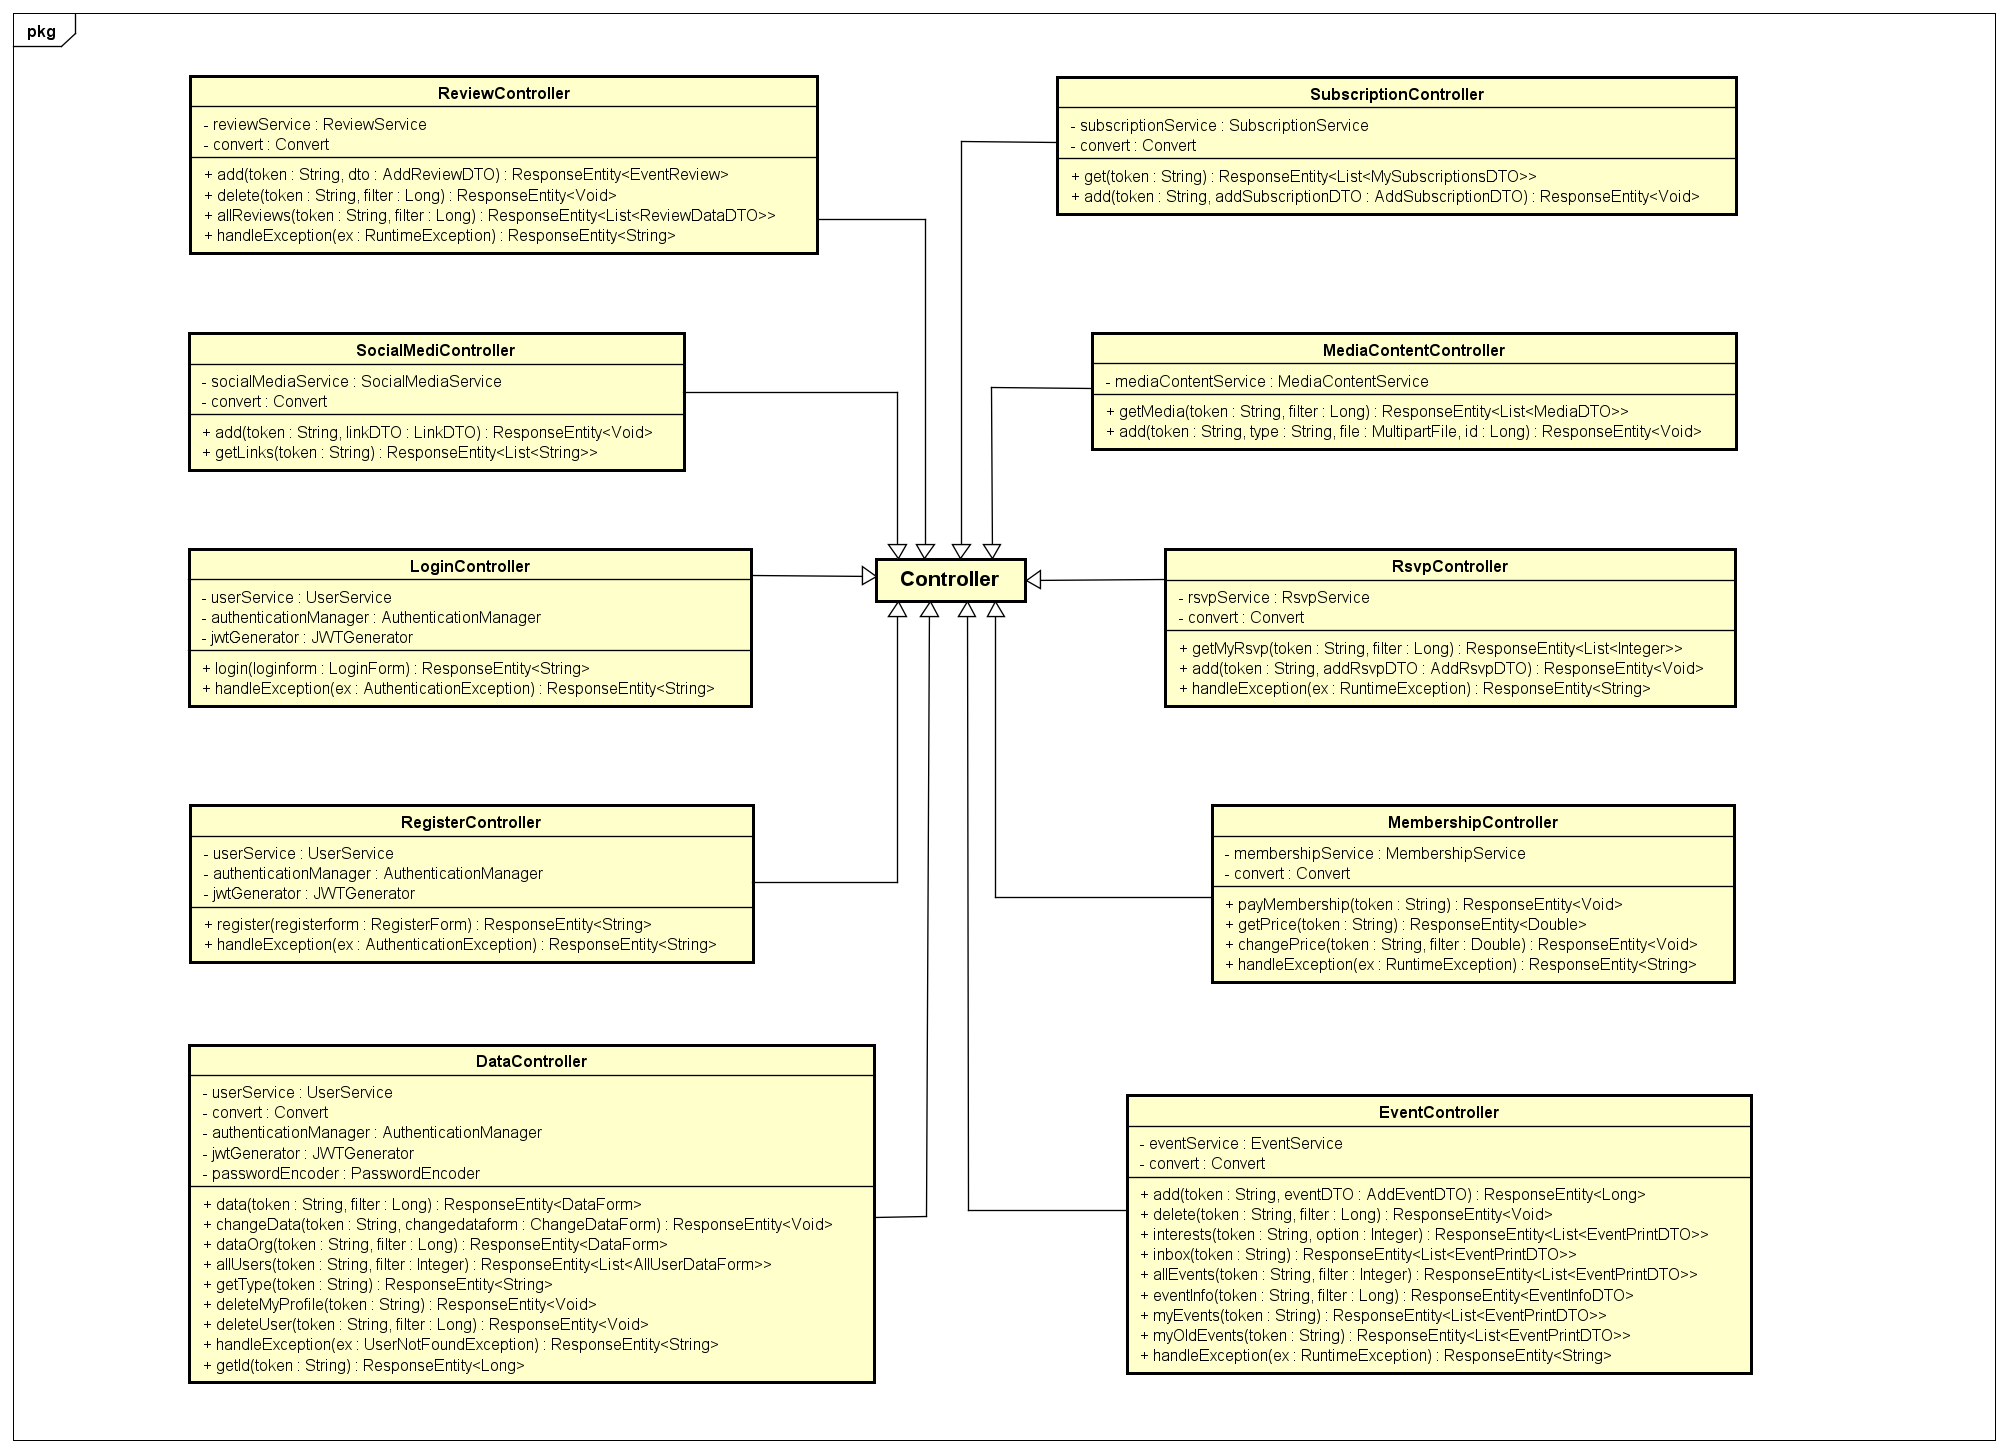
\includegraphics[width=\textwidth]{dijagrami/cd3.png} 
				\centering
				\caption{Dijagram razreda - Controllers}
				\label{cd3}
			\end{figure}
			
				\begin{figure}[H]
				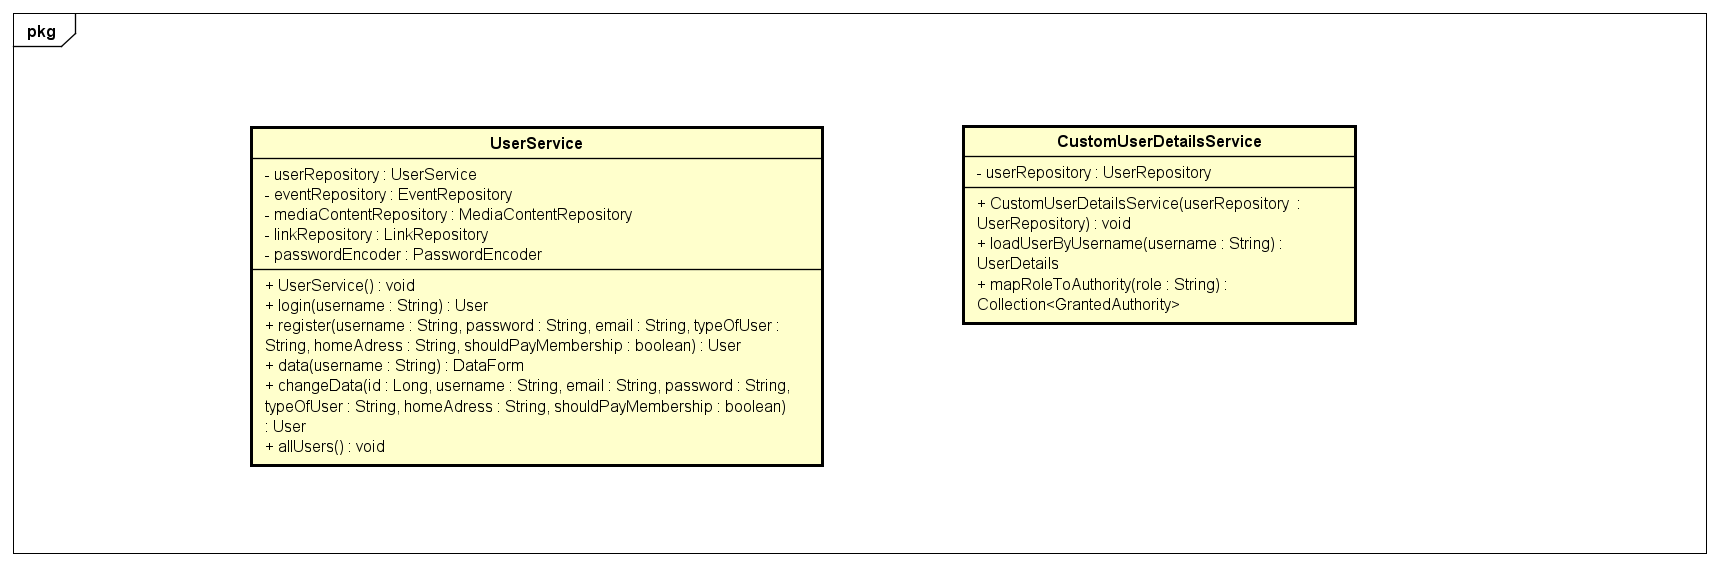
\includegraphics[width=\textwidth]{dijagrami/cd5.png} 
				\centering
				\caption{Dijagram razreda - Services}
				\label{cd5}
			\end{figure}
			
			
			\begin{figure}[H]
				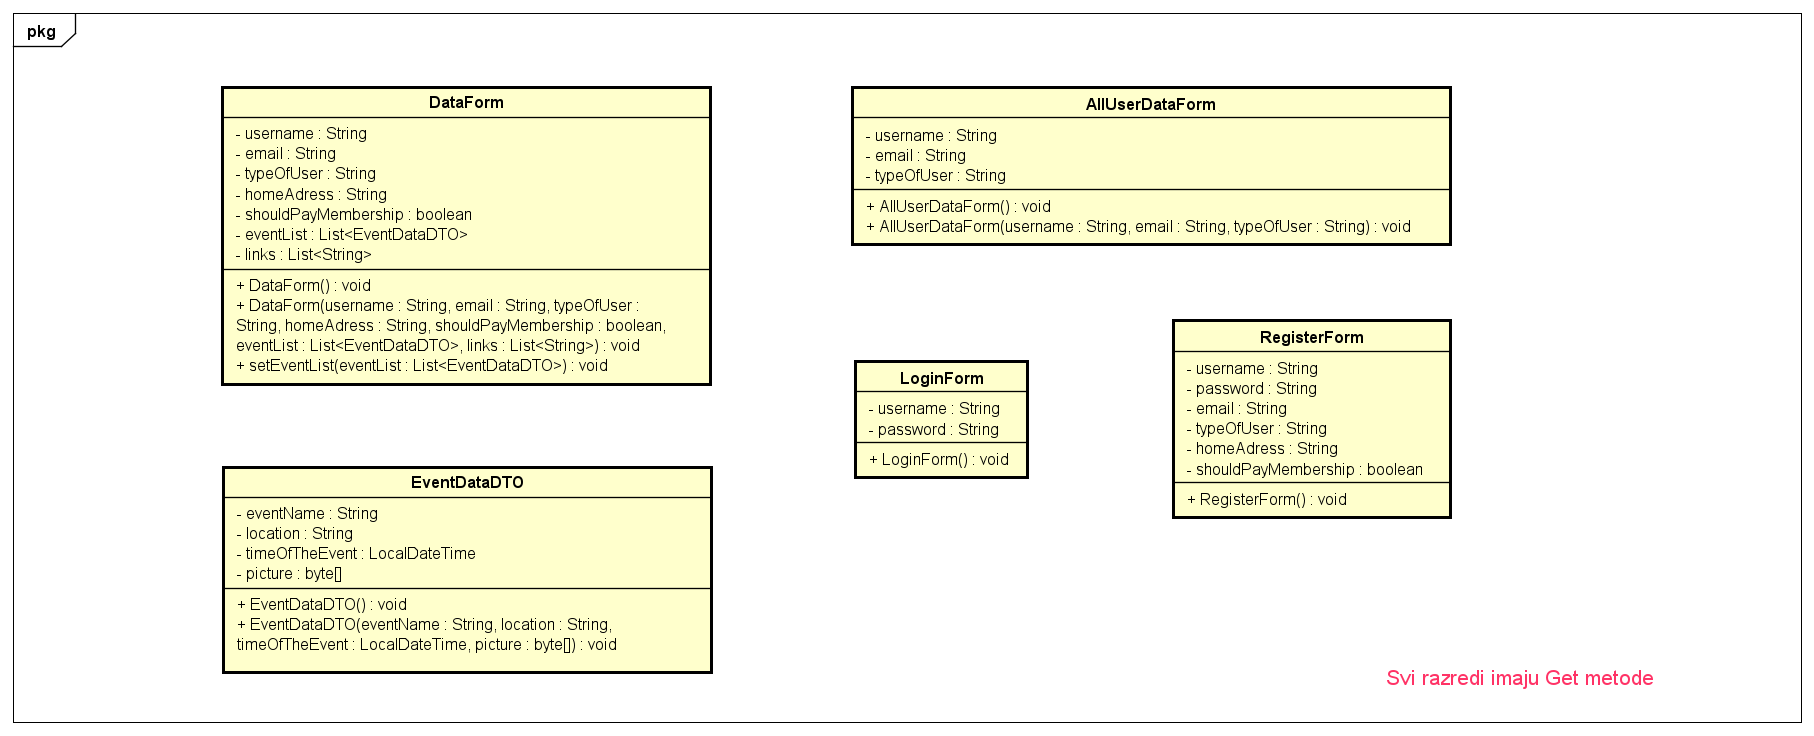
\includegraphics[width=\textwidth]{dijagrami/cd4.png} 
				\centering
				\caption{Dijagram razreda - Data transfer objects}
				\label{cd4}
			\end{figure}
			
		
			
			\newpage
			
			\begin{figure}[H]
				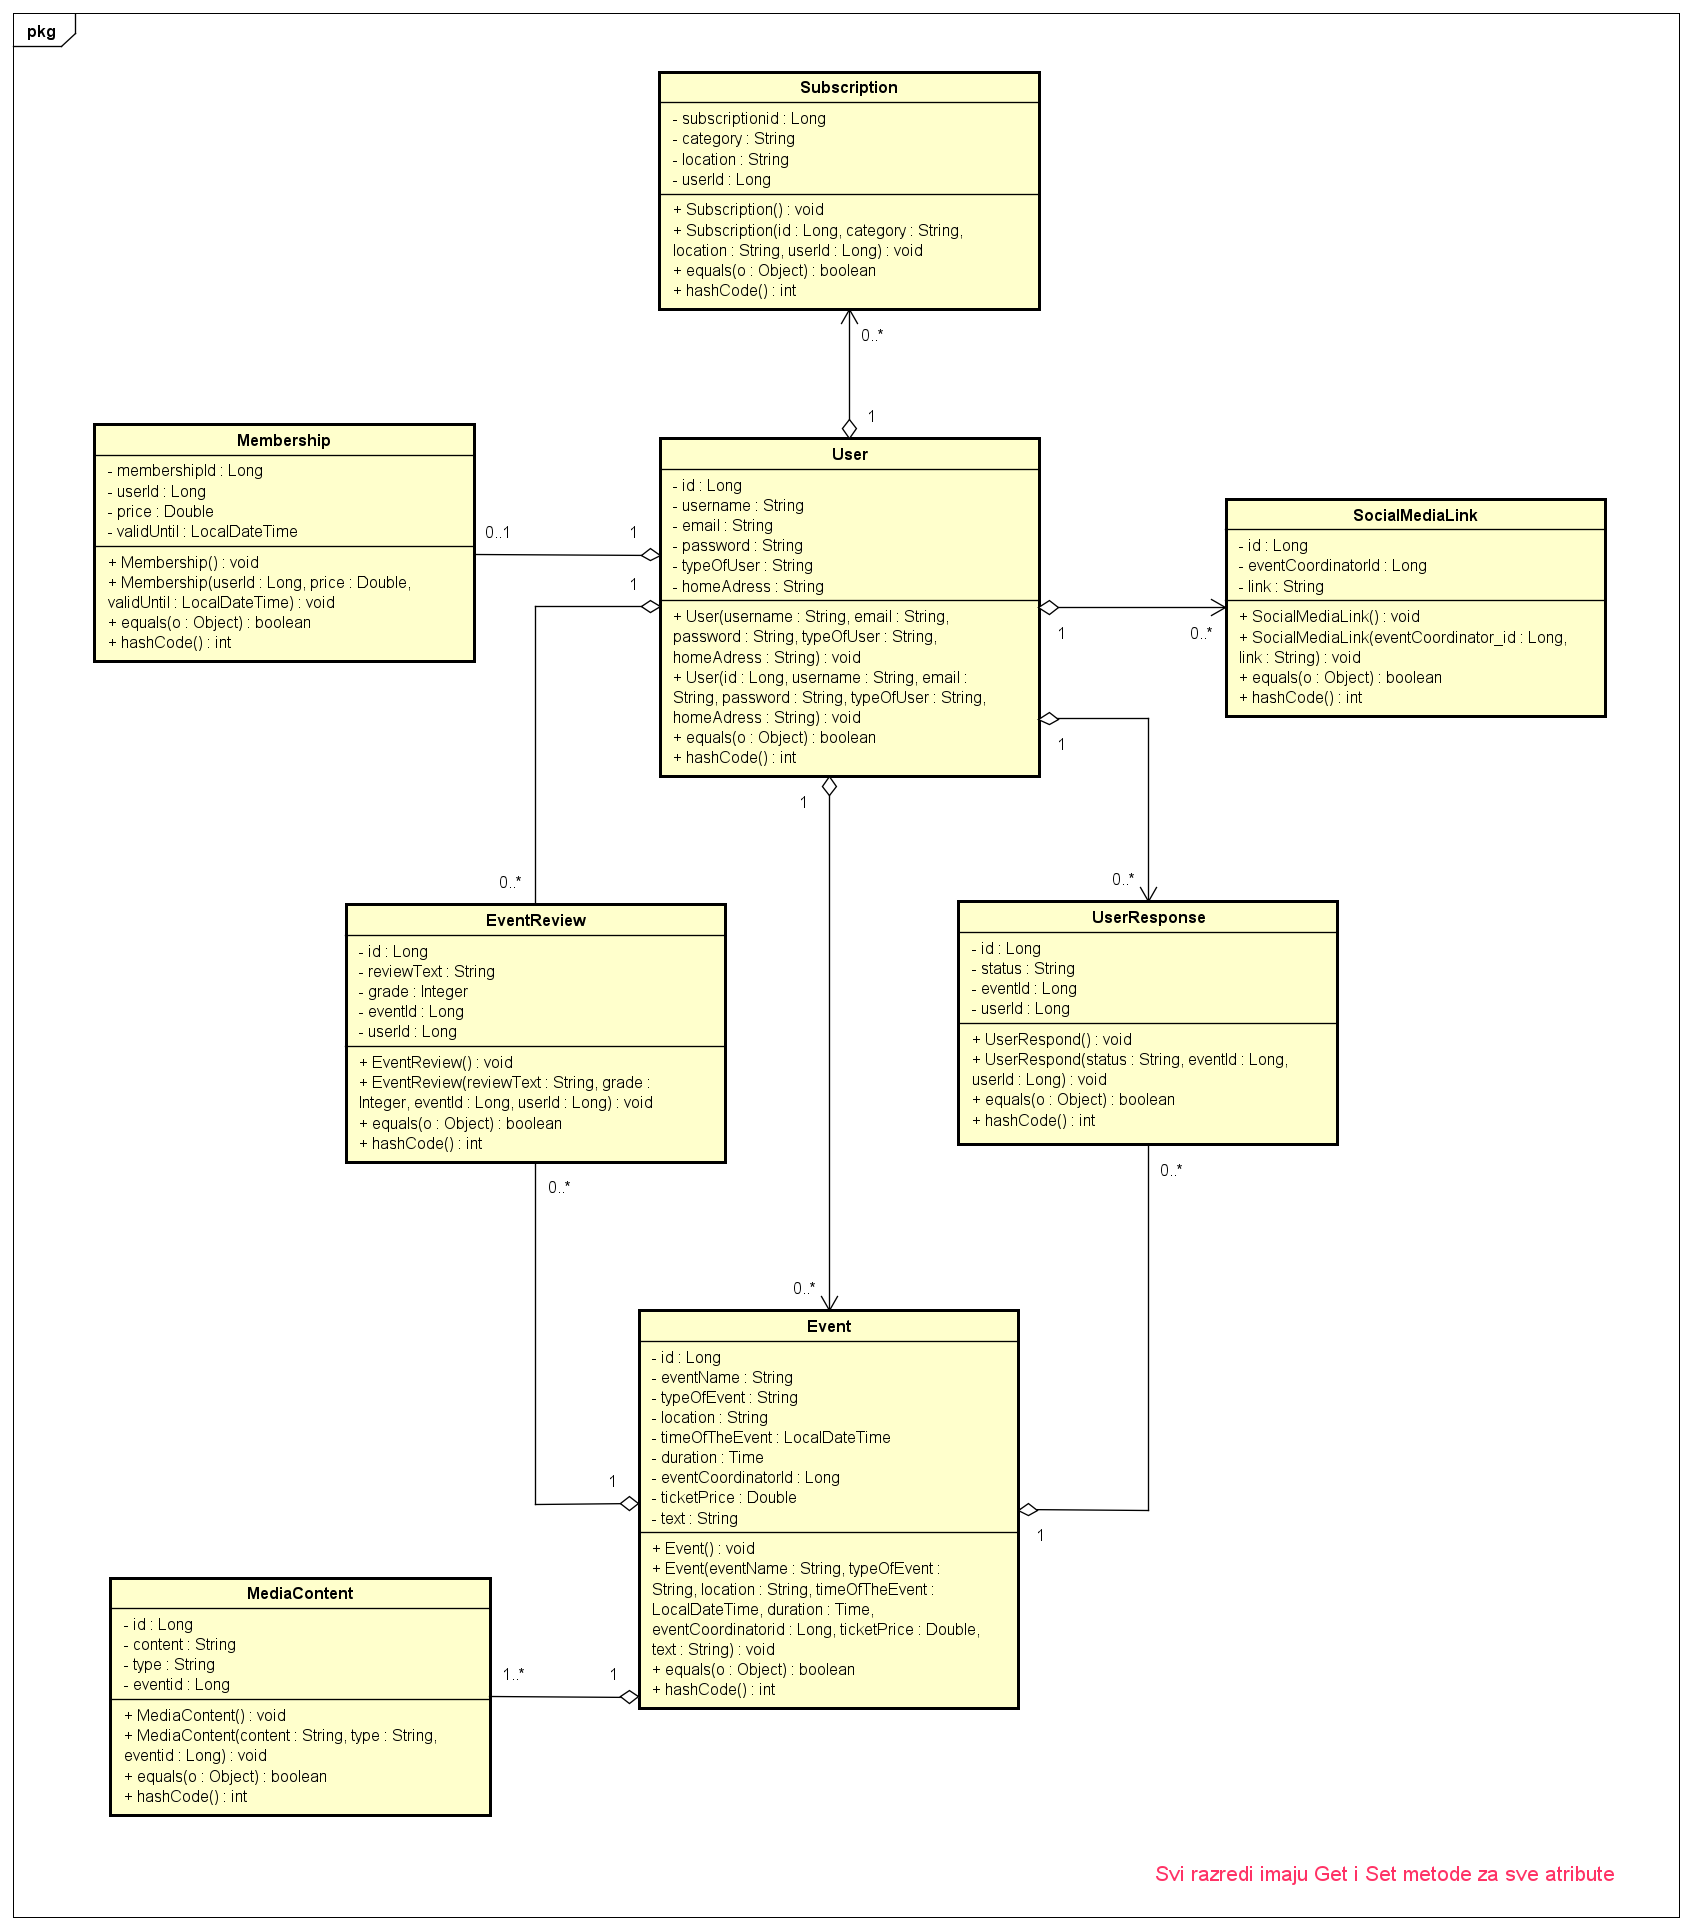
\includegraphics[width=\textwidth]{dijagrami/cd1.png} 
				\centering
				\caption{Dijagram razreda - Models}
				\label{cd1}
			\end{figure}

			\eject
		
		\section{Dijagram stanja}
			
			
			\textbf{\textit{dio 2. revizije}}\\
			
			\textit{Potrebno je priložiti dijagram stanja i opisati ga. Dovoljan je jedan dijagram stanja koji prikazuje \textbf{značajan dio funkcionalnosti} sustava. Na primjer, stanja korisničkog sučelja i tijek korištenja neke ključne funkcionalnosti jesu značajan dio sustava, a registracija i prijava nisu. }
			
			
			\eject 
		
		\section{Dijagram aktivnosti}
			
			\textbf{\textit{dio 2. revizije}}\\
			
			 \textit{Potrebno je priložiti dijagram aktivnosti s pripadajućim opisom. Dijagram aktivnosti treba prikazivati značajan dio sustava.}
			
			\eject
		\section{Dijagram komponenti}
		
			\textbf{\textit{dio 2. revizije}}\\
		
			 \textit{Potrebno je priložiti dijagram komponenti s pripadajućim opisom. Dijagram komponenti treba prikazivati strukturu cijele aplikacije.}